\documentclass[letterpaper, 12 pt, conference]{ieeeconf}
\overrideIEEEmargins
\usepackage{graphicx}
\usepackage{hyperref}
\usepackage[utf8]{inputenc}
\usepackage{fancyhdr}
\usepackage{lipsum}
\hypersetup{
    colorlinks=true,
    linkcolor=blue,
    filecolor=magenta,      
    urlcolor=cyan,
}
\pagestyle{fancy}
\fancyhead{}
\fancyfoot{}
\fancyfoot[R]{\thepage}
\pagenumbering{arabic}

\graphicspath{ {./images/} }
\title{\Huge \bf Rock-Paper-Scissors Dynamics on \\
Clustered and Random Network Structures}
\author{\huge Erik Brown, Zach Bernstein}
\begin{document}
\maketitle
\begin{abstract}
The Cyclic Lotka-Volterra model represents the dynamics of the rock-paper-scissor game in predator-prey environments. By considering this game played on a network with each node taking a locally greedy strategy, we can then determine the underlying network structure, as well as what properties affect the model's behavior. We also consider an adaptive version where the underlying network structure is changed by the agents to determine if homogeneous structures are achieved from play.
\end{abstract}
\section*{Introduction}
The Cyclic Lotka-Volterra model represents dynamics of a rock-paper-scissor game in predator-prey environments. Throughout this paper we will refer to the phrasing of this in terms of the rock-paper-scissors game, as these will be the states of our nodes in the system for computation and analysis. By considering this game played between each node connected in a network structure, we can then provide a simple mechanism for each node to determine what state they will play, and from this infer properties about the underlying network. 
The mechanism chosen is a locally greedy strategy in which each node simply plays what would beat all of its neighbors current state at each timestep. This simple mechanism was chosen as our focus for this paper is on the effects of the network played upon, so providing more sophisticated strategies for each agent leads to cloudiness between whether the emergent behavior is due to the strategy adaptations or the network itself. We also extend this to a version that allows nodes to rewire when in a converged and consistently loosing state, and compare random rewiring to rewiring that is most beneficial for each node.
\newpage
\section*{Theoretical Motivation}
Through considering a set of small toy graphs, we are able to gain intuition as to why this process may interact with the underlying network structure. For example, let us begin with a star graph, which is a network in which all nodes have degree 1 except the center node with degree N-1 (See figure 1 below for examples). If we initialize this with random states, at the first time step, all nodes except the center will simply switch to whatever beats the current state of the center. The center will change to whatever state beats most of its neighbors, but after that, we will then have the center converge to a 3 cycle between the states, and all the degree 1 nodes will also be in a 3 cycle with different state than the center, but the same state as all others. From this, we can then determine the center of the star just based on its converged behavior relative to the other nodes. This could indicate that nodes whose neighbors are all identical in state are likely to have high centrality.
\begin{figure}[ht]
    \centering
    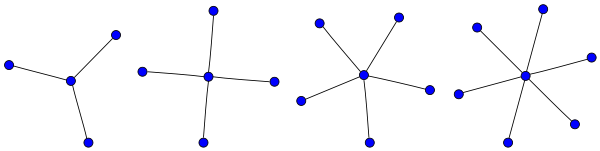
\includegraphics[width=\columnwidth]{star.png}
    \caption{Illustration of Star Graphs}
    \label{fig:star}
\end{figure}
\newpage
Another example that can be easily understood theoretically is the complete graph. This is a network is which every node is connected to every other node. In this case, whatever initial random state is most prevalent will be the most prevalent for each nodes neighborhood, and thus all nodes will switch to whatever beats this. At each timestep, the nodes will all be identical, and thus we can conclude that they all have identical neighborhoods since they only see nodes in the same state as themselves. This also converges to a 3 cycle, since there is no possibility for a "delay" that would allow one node to not change while others adapt based on their different neighborhoods. From this, we can infer that if the neighborhood of the nodes (defined as the set of all nodes who share a link with the node in question) has state distribution similar to the overall state distribution, we will see much more homogeneity in state cycle after convergence.  
\par 
Even from just these two small examples, we can see that there is intuition about what dynamics could emerge from networks that have these regular structures within their randomness. We can also hypothesize that the triangle structure will have a major role with this model, both in terms of having 3 contacting states, as well as the encouraged cycles of 3 states more than other longer converged cycles. The identification of nodes of high degree will be analyzed based on intuition about star graphs, and the identification of clusters based on the complete graph analysis will be our main metrics of interest. 
\par
If we then consider that the main convergence criteria is to cycle between the 3 states, any given node is then likely to be always winning or always loosing. From this, we can then have the node adapt to its constantly loosing situation by removing the edge from it to one of the nodes that it beating it, and instead connecting it to a random other node. This will ensure that there is always connections, since if we did not reconnect after disconnect, the graph would end in isolated nodes since we have a zero-sum game. We also consider reconnecting to a node that you are beating rather than a random one, and show that this produces a different final network structure compared to the random re-connection. 
\newpage
\section*{Network Construction}
The first networks used for analysis are created via the clustered configuration model proposed by Newman[1]. This allows us to incorporate our intuition about triangles as mentioned in the Theoretical Motivation section, as well as control the amount of clustering we have in our models which is important to real world networks such as social networks[4]. This model takes in a list of degrees for each node, as well as a list of the number of triangles each node should be included in. From these lists, the nodes are matched randomly to satisfy their degree and triangle-count constraints, which can then be used as the base for our rock-paper-scissors game. It is important to note that the sum of the degree list must be even (due to the Handshaking Lemma that must apply to all valid graph structures), and that the sum of the triangle list must be divisible by 3, since you cannot connect 1 or 2 nodes to create a triangle. 
\par
One of the primary distributions of interest for both our triangle and degree lists to be used is the discrete power law (a.k.a zipf distribution). This is inspired both for the sake of its application to real world networks as shown by Barabasi \& Albert in 1999[3], but also for its resemblance to the star graph given as a theoretical toy example. Drawing degrees from this distribution means that most of the nodes in the network will have fairly low degree, and the rest will have a significantly higher degree. Therefore, we mimic the dynamics of having select nodes with very high degree, and all others being primarily influenced by the state of these high degree nodes. Along with this, we also run tests using a constant distribution (where each node has equal degree) , as well as a discrete uniform distribution. 
\par 
While the clustered configuration model does allow for power law degree distributions through specification of the degree list, there are other mechanisms for creating a random graph that also give this distribution. In our case we look at the Barabasi \& Albert preferential attachment model[3], as well as the Dorogovtsev-Mendes model[6]. The former takes in a parameter that determines how many nodes each incoming node will attach to, thus retaining a power law degree distribution while varying the density. The latter always creates triangles, which gives opportunity to assess how important triangle structures are given that both produce scale free properties, and are thus prime candidates for comparing and contrasting results. 
\par
We also perform analysis of pure random graphs as created by the Erdos-Renyi model[5] to see how density affects the behavior. If we take a nearly complete graph (generated by letting the probability of edges existing be close to 1), we would expect behavior similar to our theoretical analysis of complete graphs. If we then continually lower this probability, we can see how low it needs to be to consistently converge to a different solution that the homogeneous strategies seen in complete graphs.  Finally we consider small world networks as generated by the Watts-Strogatz model[7] for sake of both its common use in applied settings, as well as to see how much randomness is needed to change the strategies from a deterministic model created by not reconnecting any nodes in this model. 
\section*{Methods}
The code for this project can be found \href{https://github.com/zebernst/rock-paper-scissors-network}{here}, and is created using the Python3 language. Packages used include Matplotlib, NetworkX, and NumPy along with base packages from collections and random. We created a wrapper class for our implementation of the Clustered Configuration model[1], which allowed us to specify the distribution of edges and triangles to make a graph from. These distributions were sampled from to get our edge and triangle lists, both of which were checked to ensure that the sum of degrees is even and the sum of triangles was divisible by 3 before being run through the configuration model. For the other network structures seen, basic wrappers for the generators found in NetworkX were used for generation, each of which requires parameters rather than distributions, so these can be entered directly without worry of unsatisfied constraints. 
\par
From these networks generated, we can then run our rock-paper-scissors process. For all experiments run, we decided to have initial conditions be random for each node between our 3 states. From this, we then looked at the neighborhood of each node, found its most common neighbor, and added what would beat its most common neighbor to its temporary state location. After doing so for all nodes, all nodes change state to their temporary state, which is then cleared for the next iteration. This system of updates was made to ensure simultaneous update for each node such that none have more information about future states of their neighbors than others. This is run for 25 iterations, which ensures that all dynamics converge to their cyclic steady state such that we can analyze how these patterns behave. It is important to note that 25 was chosen relatively arbitrarily, but if a network were to not converge within that time frame, an error would be thrown to indicate we needed to run for longer. This error was never thrown throughout the entirety of our testing, indicating it was sufficient. 
\par
To study what nodes converged to the same pattern, we had to see how long the period is for their cycle of states. To do so, we began from the end of our list of states for each of the 50 iterations, and worked backwards to determine period length. It is important to note that the period of the cycle must be a multiple of 3, and thus we only need to check multiples of 3. We begin by checking if the last three nodes match the three prior to that, and if so, this means we have a cycle of 3 as the converged state. If this in not the case, we then check for cycles of length 6 by seeing if the final 6 states match the 6 prior to that. We continue in power's of three until we hit cycles of length 24, as this is the longest cycle length we can check given our 50 timesteps run. If no cycle of less than 24 is found, this implies that the node has not yet converged, and thus we must run the model for longer than 50 timesteps to ensure time for convergence. 
\par
After determining what the converged behavior is of each node, we can then compare it to the behavior of other nodes to see if any patterns arise. We can do this by looking at how many nodes converged to the 3 cycle, if a majority of the nodes are of the same behavior, etc. We also extend this to a version that allows nodes to rewire when in a converged and consistently loosing state, and compare random rewiring to rewiring that is most beneficial for each node. The beneficial rewiring is done by choosing a node that is in a state you would beat to rewire to, and if none are available, instead rewire to a node that is in an identical state to yours, as either of these cases increase the "reward" of the node compared to a consistently loosing state. 
\section*{Erdos-Renyi Results}
Let us begin with the most basic random graph, which is that created by the Erdos-Renyi model. This model takes a set of nodes, and for each pair creates an edge between them independently with probability p. Therefore, if p is 0, we will have completely isolated nodes, and if p is 1, we will have the complete graph. From theoretical analysis we know that a complete graph will immediately converge to a 3 cycle where all nodes have the same state, so the main question of interest here is how low do we need to set our parameter p such that we do not see this behavior. It is clear that with a significant number of nodes, only having a few edges not exists will not greatly change the distribution of states of its neighbors compared to the global distribution, but with a significant amount of edges missing, we can find different behavior. 
\par
We began by running a binary search on our value of p to reduce our interval that our critical threshold could be in to an arbitrary level of precision. For each value of p, we run our model on a graph with 50 nodes, and run for 5 different networks to ensure that any differences are not due to the random chance of non-ideal configuration compared to our density metric of interest. We can thus empirically say that the probability of edges existing needs to be below 0.1 to have convergence to a solution that is not every node having the same behavior. It is important to note that during all of our 5 experiments for each probability tried, we found that the behavior was the same across all 5, indicating this is a hard threshold rather than having more likely or unlikely setups.  With p=0.1, we are able to get enough heterogeneity that some nodes neighborhoods are able to reflect a distribution different to that of other nodes or the entire system. This matches our initial intuition about the difference of these neighborhoods, but even then we find it surprising that it must be as low as is required. 
\section*{Barabasi-Albert Results}
The next networks of interest are Scale-Free networks where the degree distribution follows a discrete Pareto or zipf distribution. To generate these, we consider the difference between the Barabasi-Albert model and the Dorogovtsev-Mendes model. While both of these create scale free networks, the latter only creates triangles when adding nodes, so we will have higher clustering around the high degree nodes compared to the former which adds edges without concern about triangularity. Our first network is a network run with the Barabasi-Albert model with a single link between each node and the existing network. Since this creates a tree, and the high degree hubs locally represent structure similar to the star graph, we find that similar dynamics appear. 
\begin{figure}[ht]
    \centering
    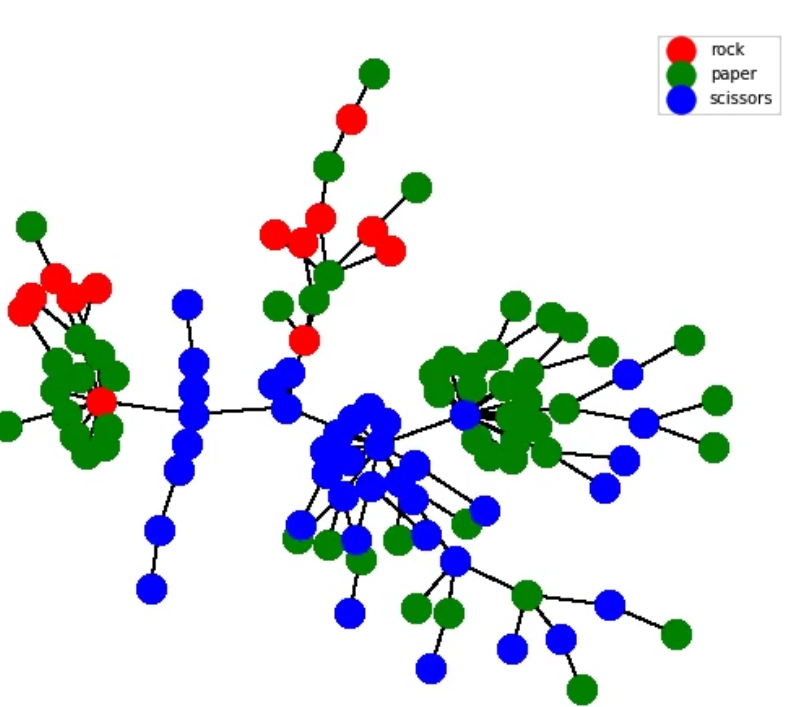
\includegraphics[width=\columnwidth]{ba_net.png}
    \caption{Converged Strategies of BA Scale-Free Network}
    \label{fig:ba net}
\end{figure}

For each of the small sets of nodes clumped together, we know that this is a node of high degree surrounded by nodes of relatively low degree. For the clumps on the left and right side, we see a red or blue node surrounded by many green nodes indicating similar dynamics to the star graph. For the third clump that is primarily blue nodes, we expect that this is because the central node in the cluster on the right is connected to the center of this node, and at the beginning this slight change caused both the center and leaves to optimize their state to paper, thus leading to homogeneity in this. It is also important to note that even with our constant that this model only creates trees, we still see that the dynamics do not perfectly match that analyzed theoretically due to things such as the random initial conditions or situations where the high degree nodes happen to have a link to each other. 
\section*{Dorogovtsev-Mendez Results}
To consider how having a non-tree structure affects the dynamics when we still have our central nodes due to the scale-free property, we turn to the Dorogovtsev-Mendes model. This model was run for 6 generations, which is the only parameter of the model given that a specific number of nodes is not taken in, but rather a number of generations from a base graph of $K_3$. The following figure shows that because we have much more connection, the "cloud" of nodes in the neighborhood around the high degree nodes is much more connected, and thus all nodes in this set have similar neighborhood, leading to dynamics closer to a local version of the complete graph. 
\begin{figure}[ht]
    \centering
    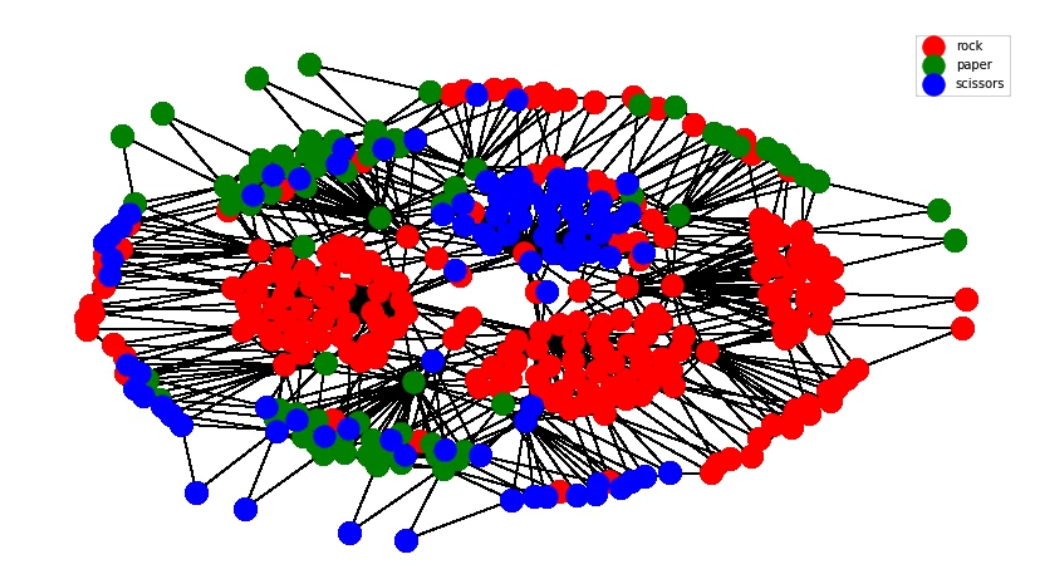
\includegraphics[width=\columnwidth]{dm.png}
    \caption{Converged Strategies of DM Scale-Free Network}
    \label{fig:dm net}
\end{figure}
As we can see because of the high amount of clustering in each of the groups seen visually, we find that if we only look at one of these clusters, there is a uniform strategy as if this cluster was a complete graph. This makes sense because even though the high degree nodes are within the cluster just like with the Barabasi-Albert model, the non-central nodes were not connected to each other, whereas here they must be since the model runs by creating a triangle with an existing edge at every point, so it is impossible to connect to only the high degree node. It is important to note that there is some "noise" in these clusters created by nodes who are connected between multiple clusters. It is in this case that these nodes' neighborhoods are not reflective of the neighborhoods of the cluster since they are split between multiple state distributions, and thus there is potential to identify these nodes more than the high degree based on how different they are compared to their "assigned" cluster. 
\section*{Adaptive Network Results}
For our extension with changing the network structure, we begin by letting nodes who are loosing after convergence disconnect from a node they are loosing to and instead connect randomly to a new node. With this, our main question is whether or not the resulting network is nearly purely random, as with all of the random re-connections, we would expect that this is equivalent to randomly determining if edges exist or not, which is the Erdos-Renyi generator. We can therefore test this by determining if we end up with a degree distribution that approximately follows a Poisson distribution since each edge existing should be an independent Bernoulli variable, and thus we have a binomial distribution, which converges in distribution to a Poisson as the number of edges goes to infinity due to the Poisson limit theorem.
\par
Since we only allow each node to disconnect 1 edge at each round, we begin by considering the Clustered Configuration model[1] with 200 nodes. We use a uniform distribution for our degree list as well as our triangle list, as this gives a relatively regular structure which does not require a significant number of rewiring steps to potentially approach our Poisson degree distribution. The following figure shows the resulting distribution in orange, as well as an overlaid Poisson distribution, which shows relatively good fit. 

\begin{figure}[ht]
    \centering
    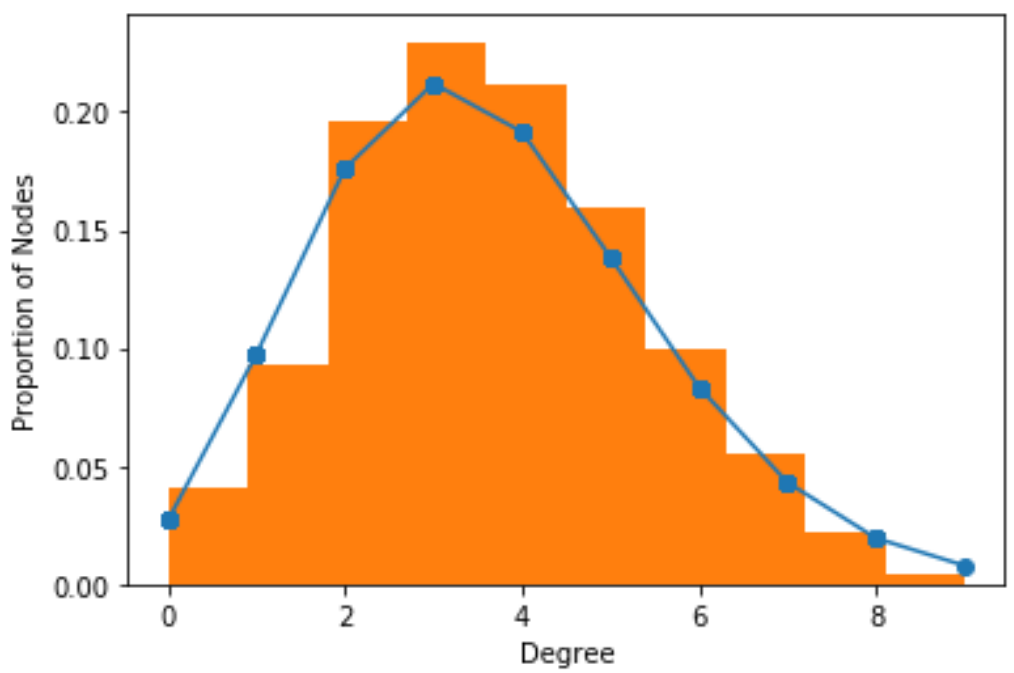
\includegraphics[width=\columnwidth]{ccf.png}
    \caption{Adaptive Clustered Configuration Degree Distribution}
    \label{fig:cc}
\end{figure}
\newpage
Since this fits well, we then consider a distribution that is significantly more heterogeneous to determine if it still approaches this distribution. For this we turn again to the Barabasi-Albert model with 2 connections at each timestep and 200 nodes. This produces the following degree distribution which while not quite as well fit due to the remaining high degree node at the end, is closer than the initial power law degree distribution which is significantly different. 
\begin{figure}[ht]
    \centering
    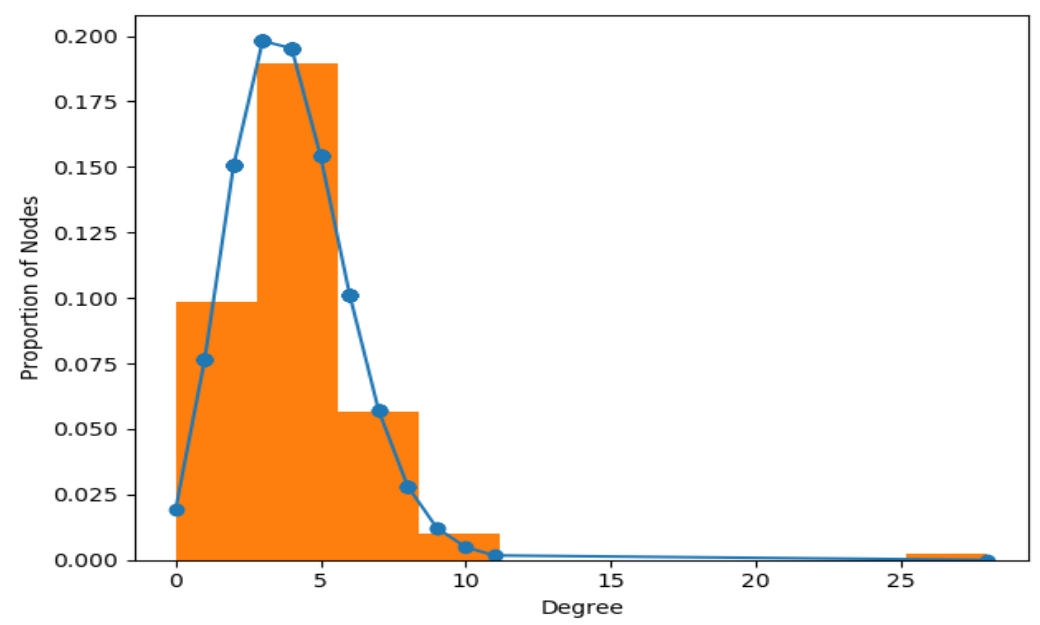
\includegraphics[width=\columnwidth]{ba.png}
    \caption{Adaptive Clustered Configuration Degree Distribution}
    \label{fig:ba}
\end{figure}
\newpage
If we then change this to allow for nodes to identify where they should reconnect such that they maximize their winnings, we expect that we should not reach a Poisson distribution. This is because by reconnecting to specific nodes, our connections should be between clusters of like nodes more than to random nodes that are not of interest. This is indeed what we see as shown in the following figure that was generated using the same setup from the clustered configuration model as prior. 
\begin{figure}[ht]
    \centering
    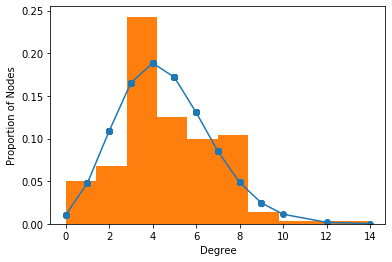
\includegraphics[width=\columnwidth]{degree_dist.png}
    \caption{Non-random Adaptive Clustered Configuration Degree Distribution}
    \label{fig:nrcc}
\end{figure}
\section*{Conclusion}
Overall, we see that while we are still able to find some interesting properties, we do not have nearly as much information to be gained compared to the theoretical networks analysed. While this does make sense given that the information gained from analysis is fully dependent on complete knowledge of the network structures, we feel that perhaps we would be able to tease more out with agents that do not conform to our locally greedy strategy. Perhaps taking an evolutionary game theory approach that allows the network structure to have a bigger effect on the behavior of the nodes could help us clue into this interaction, but we still feel that this may cloud the importance of the network relative to the importance of how the agents choose their states and strategies.
\addtolength{\textheight}{-9cm}  
\newpage
\begin{thebibliography}{99}
\bibitem{c1}
M.E.J. Newman (2009) Random Graphs with Clustering 
\bibitem{c2}
György Szabó, Attila Szolnoki, Rudolf Izsák (2004)
Rock-Scissors-Paper Game on Regular Small-World Networks
\bibitem{c3} 
Albert-Laszlo Barabasi $\&$ Reka Albert. (1999) Emergence of scaling in random networks
\bibitem{c4}
Nina Mishra et. al (2007) Clustering Social Networks
\bibitem{c5}  
P. Erdos $\&$ A. Renyi (1960) On the evolution of random graphs.
\bibitem{c6}
S.N. Dorogovtsev $\&$ J.F.F. Mendes (2001) Evolution of networks
\bibitem{c7} 
Duncan J. Watts $\&$ Steven H. Strogatz (1998) Collective dynamics of `small-world' networks
\end{thebibliography}
\end{document}
